% Block 1: Sicherheit
\begin{frame}{Hitze verstehen}
\begin{columns}[T]
    \begin{column}{0.58\textwidth}
        \small
        \begin{itemize}\setlength{\itemsep}{3mm}
            \item - Der Pinecil kann sehr heiß werden bis zu 450 °C
            \item - Spitze nie berühren oder anfassen!
            \item - Nur in der Halterung oder auf der Matte ablegen.
        \end{itemize}
        \normalsize
    \end{column}
    \begin{column}{0.42\textwidth}
        \centering
        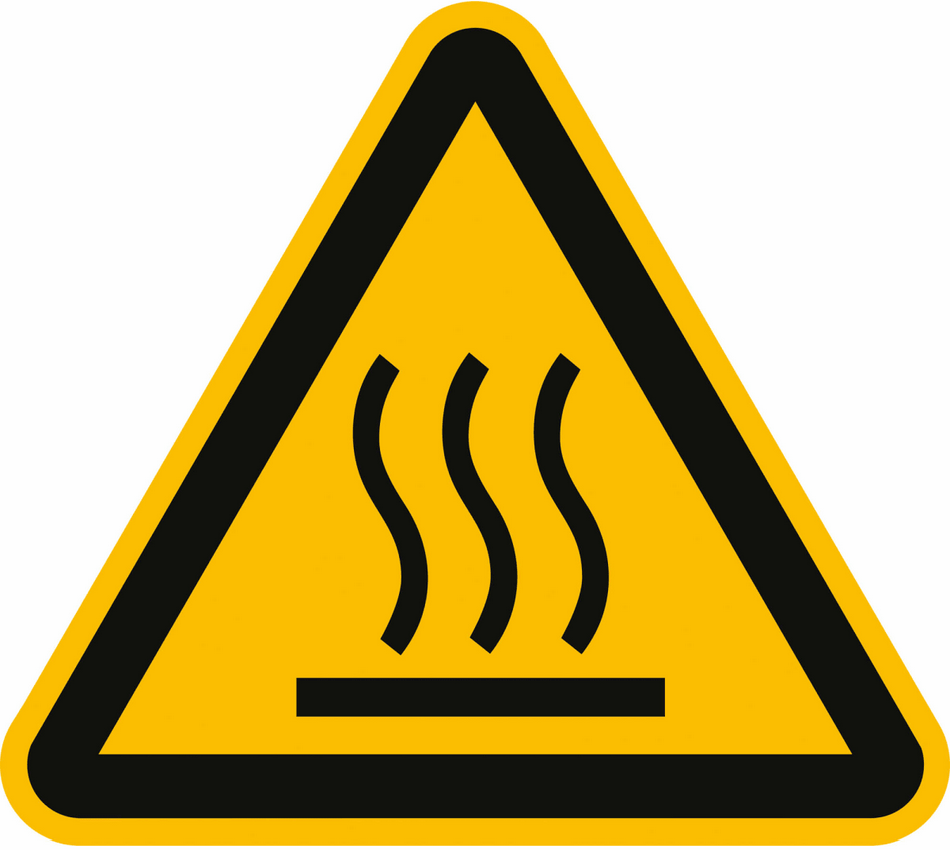
\includegraphics[width=\linewidth,keepaspectratio]{2.0.0.0_content/assets/bilder/Warnzeichen.png}
    \end{column}
\end{columns}
\end{frame}

\begin{frame}{Arbeitsplatz}
\begin{columns}[T]
    \begin{column}{0.58\textwidth}
        \small
        \begin{itemize}\setlength{\itemsep}{3mm}
            \item Aufgeräumt und gut beleuchtet
            \item Wärmeresistente Unterlage
            \item Kabel sicher führen
        \end{itemize}
        \normalsize
    \end{column}
    \begin{column}{0.42\textwidth}
        \centering
        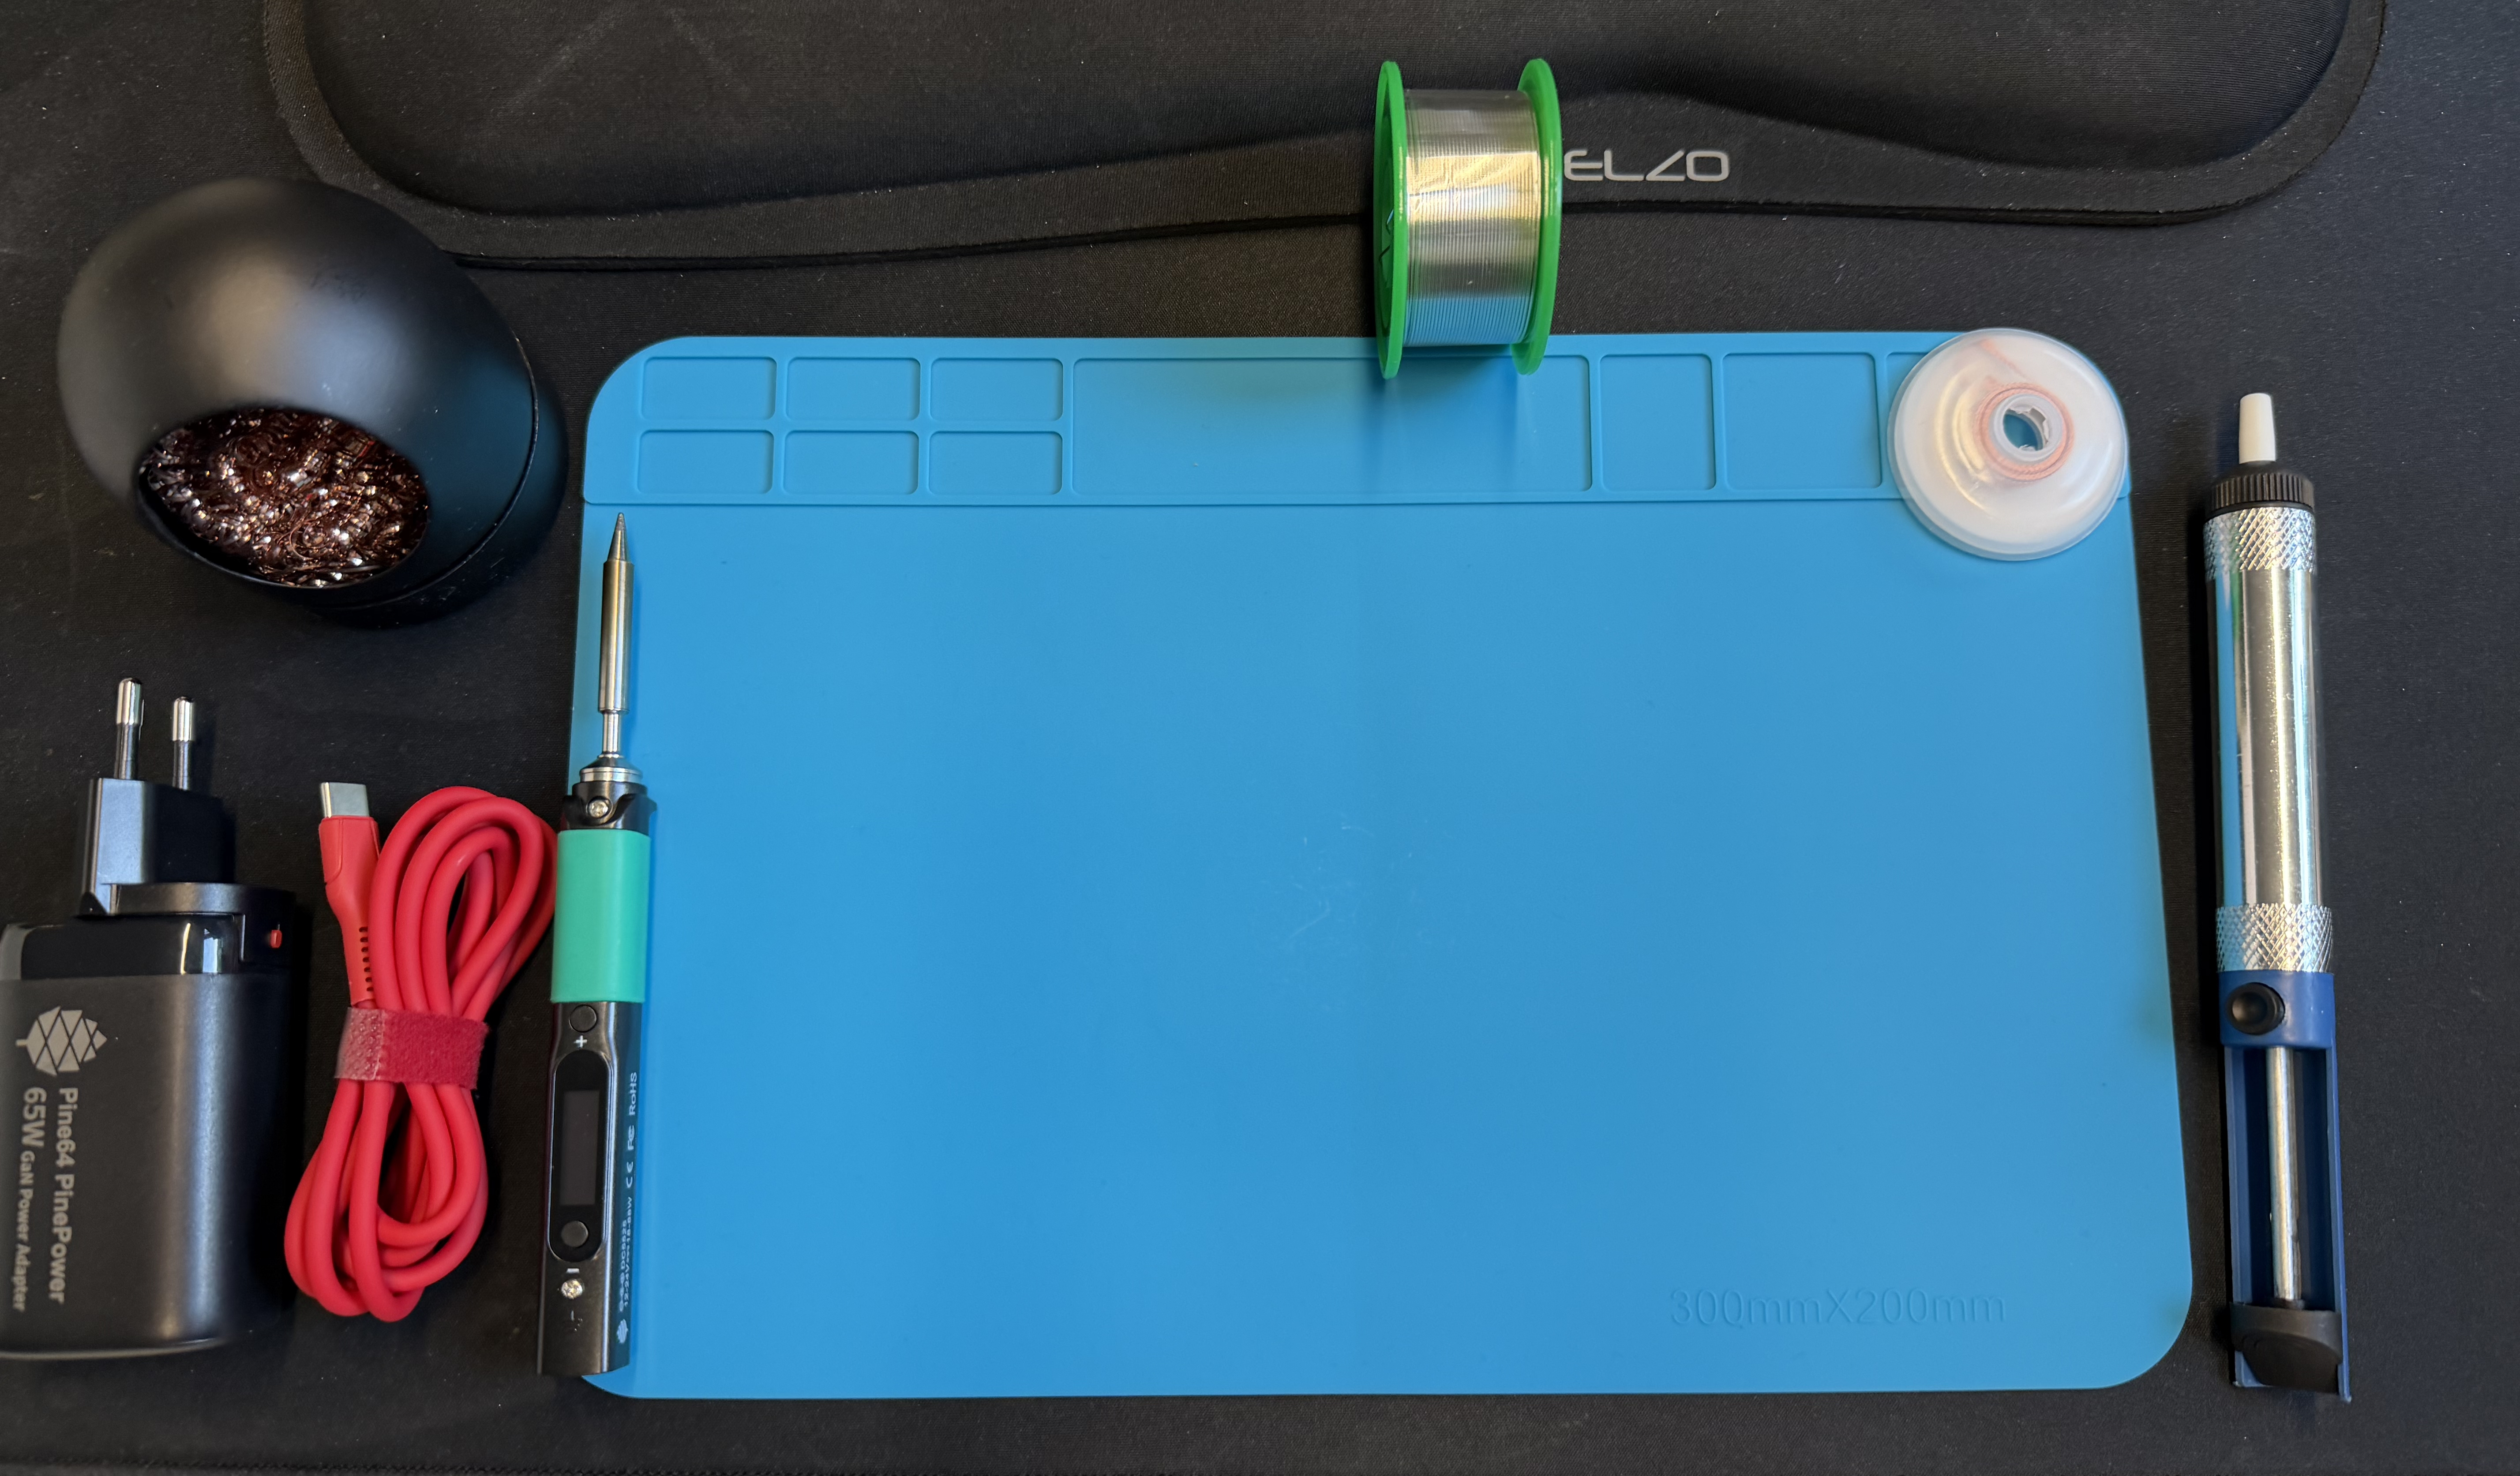
\includegraphics[width=\linewidth,keepaspectratio]{2.0.0.0_content/assets/bilder/setup.jpg}
    \end{column}
\end{columns}
\end{frame}

\begin{frame}{Dämpfe und Luft}
\begin{itemize}\setlength{\itemsep}{3mm}
    \item - Gut lüften
    \item - Rauch nicht einatmen
    \item - Absaugung bei Bedarf
\end{itemize}
\end{frame}

\begin{frame}{Schutz und Verhalten}
\begin{itemize}\setlength{\itemsep}{3mm}
    \item - Schutzbrille bei Drahtarbeiten
    \item - Keine Getränke an der Lötstelle
    \item - Nicht mit Kolben herumlaufen
\end{itemize}
\end{frame}